\documentclass{article}

% packages
  % basic stuff for rendering math
  \usepackage[letterpaper, top=1in, bottom=1in, left=1in, right=1in]{geometry}
  \usepackage[utf8]{inputenc}
  \usepackage[english]{babel}
  \usepackage{amsmath} 
  \usepackage{amssymb}
  % \usepackage{amsthm}

  % extra math symbols and utilities
  \usepackage{mathtools}        % for extra stuff like \coloneqq
  \usepackage{mathrsfs}         % for extra stuff like \mathsrc{}
  \usepackage{centernot}        % for the centernot arrow 
  \usepackage{bm}               % for better boldsymbol/mathbf 
  \usepackage{enumitem}         % better control over enumerate, itemize
  \usepackage{hyperref}         % for hypertext linking
  \usepackage{fancyvrb}          % for better verbatim environments
  \usepackage{newverbs}         % for texttt{}
  \usepackage{xcolor}           % for colored text 
  \usepackage{listings}         % to include code
  \usepackage{lstautogobble}    % helper package for code
  \usepackage{parcolumns}       % for side by side columns for two column code
  

  % page layout
  \usepackage{fancyhdr}         % for headers and footers 
  \usepackage{lastpage}         % to include last page number in footer 
  \usepackage{parskip}          % for no indentation and space between paragraphs    
  \usepackage[T1]{fontenc}      % to include \textbackslash
  \usepackage{footnote}
  \usepackage{etoolbox}

  % for custom environments
  \usepackage{tcolorbox}        % for better colored boxes in custom environments
  \tcbuselibrary{breakable}     % to allow tcolorboxes to break across pages

  % figures
  \usepackage{pgfplots}
  \pgfplotsset{compat=1.18}
  \usepackage{float}            % for [H] figure placement
  \usepackage{tikz}
  \usepackage{tikz-cd}
  \usepackage{circuitikz}
  \usetikzlibrary{arrows}
  \usetikzlibrary{positioning}
  \usetikzlibrary{calc}
  \usepackage{graphicx}
  \usepackage{caption} 
  \usepackage{subcaption}
  \captionsetup{font=small}

  % for tabular stuff 
  \usepackage{dcolumn}

  \usepackage[nottoc]{tocbibind}
  \pdfsuppresswarningpagegroup=1
  \hfuzz=5.002pt                % ignore overfull hbox badness warnings below this limit

% Custom Environments
  \newtcolorbox[auto counter, number within=section]{example}[1][]
  {
    colframe = orange!25,
    colback  = orange!10,
    coltitle = orange!20!black,  
    breakable, 
    title = \textbf{Question \thetcbcounter ~(#1)}
  }
  \newtcolorbox[auto counter, number within=section]{definition}[1][]
  {
    colframe = yellow!25,
    colback  = yellow!10,
    coltitle = yellow!20!black,  
    breakable, 
    title = \textbf{Definition \thetcbcounter ~(#1)}
  } 
  \newtcolorbox[auto counter, number within=section]{society}[1][]
  {
    colframe = yellow!25,
    colback  = yellow!10,
    coltitle = yellow!20!black,  
    breakable, 
    title = \textbf{Society \thetcbcounter}
  }
  \newtcolorbox[auto counter, number within=section]{politics}[1][]
  {
    colframe = red!25,
    colback  = red!10,
    coltitle = red!20!black,  
    breakable, 
    title = \textbf{Politics \thetcbcounter ~(#1)}
  }
  \newtcolorbox[auto counter, number within=section]{legal}[1][]
  {
    colframe = blue!25,
    colback  = blue!10,
    coltitle = blue!20!black,  
    breakable, 
    title = \textbf{Legal \thetcbcounter ~(#1)}
  } 
  \newtcolorbox[auto counter, number within=section]{finance}[1][]
  {
    colframe = green!25,
    colback  = green!10,
    coltitle = green!20!black,  
    breakable, 
    title = \textbf{Finance \thetcbcounter ~(#1)}
  } 
  \newtcolorbox[auto counter, number within=section]{religion}[1][]
  {
    colframe = violet!25,
    colback  = violet!10,
    coltitle = violet!20!black,  
    breakable, 
    title = \textbf{Religion \thetcbcounter ~(#1)}
  }
  \newtcolorbox[auto counter, number within=section]{technology}[1][]
  {
    colframe = violet!25,
    colback  = violet!10,
    coltitle = violet!20!black,  
    breakable, 
    title = \textbf{Technology \thetcbcounter ~(#1)}
  }

  \BeforeBeginEnvironment{example}{\savenotes}
  \AfterEndEnvironment{example}{\spewnotes}
  \BeforeBeginEnvironment{lemma}{\savenotes}
  \AfterEndEnvironment{lemma}{\spewnotes}
  \BeforeBeginEnvironment{theorem}{\savenotes}
  \AfterEndEnvironment{theorem}{\spewnotes}
  \BeforeBeginEnvironment{corollary}{\savenotes}
  \AfterEndEnvironment{corollary}{\spewnotes}
  \BeforeBeginEnvironment{proposition}{\savenotes}
  \AfterEndEnvironment{proposition}{\spewnotes}
  \BeforeBeginEnvironment{definition}{\savenotes}
  \AfterEndEnvironment{definition}{\spewnotes}
  \BeforeBeginEnvironment{exercise}{\savenotes}
  \AfterEndEnvironment{exercise}{\spewnotes}
  \BeforeBeginEnvironment{proof}{\savenotes}
  \AfterEndEnvironment{proof}{\spewnotes}
  \BeforeBeginEnvironment{solution}{\savenotes}
  \AfterEndEnvironment{solution}{\spewnotes}
  \BeforeBeginEnvironment{question}{\savenotes}
  \AfterEndEnvironment{question}{\spewnotes}
  \BeforeBeginEnvironment{code}{\savenotes}
  \AfterEndEnvironment{code}{\spewnotes}

  \definecolor{dkgreen}{rgb}{0,0.6,0}
  \definecolor{gray}{rgb}{0.5,0.5,0.5}
  \definecolor{mauve}{rgb}{0.58,0,0.82}
  \definecolor{lightgray}{gray}{0.93}

  % default options for listings (for code)
  \lstset{
    autogobble,
    frame=ltbr,
    language=C,                           % the language of the code
    aboveskip=3mm,
    belowskip=3mm,
    showstringspaces=false,
    columns=fullflexible,
    keepspaces=true,
    basicstyle={\small\ttfamily},
    numbers=left,
    firstnumber=1,                        % start line number at 1
    numberstyle=\tiny\color{gray},
    keywordstyle=\color{blue},
    commentstyle=\color{dkgreen},
    stringstyle=\color{mauve},
    backgroundcolor=\color{lightgray}, 
    breaklines=true,                      % break lines
    breakatwhitespace=true,
    tabsize=3, 
    xleftmargin=2em, 
    framexleftmargin=1.5em, 
    stepnumber=1
  }

% Page style
  \pagestyle{fancy}
  \fancyhead[L]{Mesopotamians}
  \fancyhead[C]{Muchang Bahng}
  \fancyhead[R]{Spring 2024} 
  \fancyfoot[C]{\thepage / \pageref{LastPage}}
  \renewcommand{\footrulewidth}{0.4pt}          % the footer line should be 0.4pt wide
  \renewcommand{\thispagestyle}[1]{}  % needed to include headers in title page

\begin{document}

\title{Mesopotamians}
\author{Muchang Bahng}
\date{Spring 2024}

\maketitle
\tableofcontents
\pagebreak

  In here I talk about the development of two of the cradles of civilization: the Mesopotamians and Egyptians. I conglomorated them into a single set of notes since they were quite interdependent and were physically the same. We start off with the civilizations in the \textbf{Fertile Crescent}, which is shown below. 

  \begin{figure}[H]
    \centering 
    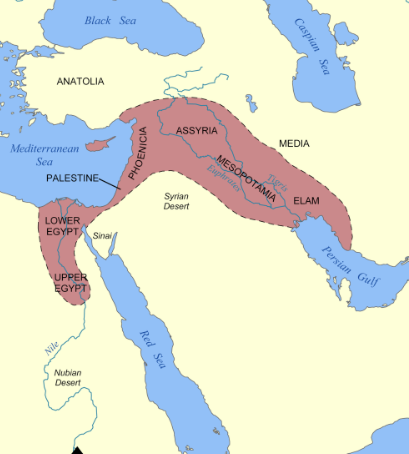
\includegraphics[scale=0.4]{img/fertile_crescent.png}
    \caption{The Fertile Crescent is a crescent-shaped region in the Middle East, spanning modern-day Iraq, Syria, Lebanon. As we will see later, the advance of agriculture made this region a great place to settle. } 
    \label{fig:fertile_crescent}
  \end{figure}

  But to talk about civilizations, we must first define what it is and differentiate it from other forms of human organization like hunter gatherers, tribes, or cavemen. The rigorous definition is often debated, so we will stick with the following rudimentary one. 

  \begin{definition}[Civilization]
    A \textbf{civilization} is a complex society characterized by the following 
    \begin{enumerate}
      \item \textbf{Urban development} is the process of creating cities. 
      \item \textbf{Social stratification} is the division of society into classes. 
      \item A form of \textbf{government} is the system by which a state or community is controlled. 
      \item \textbf{Symbolic communication forms} like writing.
    \end{enumerate}
  \end{definition}

  A more rudimentary version of civilization is called a \textbf{culture}. 

  \begin{definition}[General Timeline]
    The following is general taxonomy of human history. 
    \begin{enumerate} 
      \item (-3000 BCE) The \textbf{Stone age} is a prehistoric period during which stone was widely used to make stone tools, lasting for approximately 3.4 million years. It is divided into 3 subcategories. 
        \begin{enumerate}
          \item (- 9000 BCE) The \textbf{Paleolithic era} is the primitive use of stones. 
          \item The \textbf{Mesolithic era} is transitionary period. 
          \item (9000 - 3000 BCE) The \textbf{Neolithic era} is the final stage characterized by agriculture. 
        \end{enumerate}
      \item (3000 - 1200 BCE) The \textbf{Bronze age} is characterized by the use of bronze tools, the use of writing in some areas, and the features of urban civilization. 
      \item (1200 - 550 BCE) The \textbf{Iron age} evolved from bronze to iron. 
    \end{enumerate}
  \end{definition}

\section{Pre-Sumerian Hunter Gatherers}

  \subsection{Hunter Gatherers}

    The \textbf{Stone Age} is a prehistoric period during which stone was widely used to make stone tools, lasting for approximately 3.4 million years.\footnote{The period of time before civilization developed is called \textbf{prehistory}. } The majority of the Stone age was spent in the \textbf{Paleolithic era}, where humans were hunter gatherers, which were bands of humans, often an extended family but growing up to 100 people, who traveled around for food and shelter. Guided by their knowledge in geography, each group would travel across a span of land hundreds of miles wide, following the migration of animals, the growth of plants, and the changing of seasons. Due to the fertile land that allowed wildlife and vegetation to grow in the Fertile Crescent, most cultures originated from Mesopotamia and Egypt. 

    Note that this was inherently limited. First, with a limited supply of food in each area, groups cannot be unbounded in size. Larger groups meant more traveling, and at some point you would have to travel at an unsustainable pace, which is why there was an inherent limit in these sizes. 

    Even at this rudimentary stage, there was some specialization of labor, with the first example being that males, who were physically stronger, would hunt, and females would gather vegetation and take care of children. This allowed for a more efficient use of resources. With individuals specializing in their tasks, one would think that \textbf{bartering}, the practice of trading good and services, would have been common. However, there is not much evidence for this. Rather, one a group had secured a resource, it would simply be distributed within the tribe. 

    Furthermore, there was no social stratification, as everyone was equal. There may have been leaders who directed the group, but they were not considered superior to others. Similarly, there was no concept of private property. 

    Interactions between two tribes are not well known, and it is hard to tell how territorial they may have been. The main reason would have been for a competition of resources, but these communities may have traveled rotationally so that they don't bump into each other. 

  \subsection{Neolithic Era}

    \begin{technology}[Agriculture is Discovered]
      However, around 9000 BCE, the \textbf{Neolithic era} began, where various hunter gatherers who discovered agriculture began to separate from their main groups and begin settlements, staring with those in the Fertile Crescent and others following rapidly. This had several consequences. 
    \end{technology}

    \begin{society}[Population Growth]
      There was an explosive population growth. Since they were not limited by the ability to travel and were self-sustaining, they could feed more mouths and often had a surplus of food. 
    \end{society}

    \begin{finance}[Private Property]
      With settlements, households began to own private property by building their own shelters (with adobe) on claimed land. More sophisticated tools like clay pottery were also developed. 
    \end{finance}

    \begin{finance}[Social Inequality]
      The domestication and possession of large animals resulted in a dramatic increase in social inequality since it allowed competition between households and resulted in inherited inequalities of wealth. This led to tribal leaders, chiefs, or small elite groups of people (though this was not pronounced until the Bronze age).\footnote{This would be the birth of primitive governments.} 
    \end{finance}

    \begin{finance}[Sophsitication of Bartering]
      With households working in each area of labor, the surplus of grain and cattle allowed more sophisticated forms of bartering, though a common currency was not established yet and values can still be negotiated. 
    \end{finance}

    \begin{finance}[First Bookkeeping Practices]
      Bookkeeping of agricultural production was established. At this point writing may not have been invented yet, and so farmers would take clay tokens and store them in pots as a method of accounting. This gave rise to the first accounting practices in humanity that tracked whether surplus had been gained. 
    \end{finance}

    Over the next millennia, these settlements would grow at this pace to become city-states, and Mesopotamia would be scattered with independent city-states in this \textit{Chalcolithic period}. Major city-states, whose names will become important, were Uruk, Ur, Kish and Eridu. 

\section{Uruk and Jemdet Nasr Periods (3500-2900 BCE)}

    Around 3500 BCE, the ancient \textbf{Sumerians} (whose origin is not well known but was believed to have migrated) settled into the city of Uruk Mesopotamia near the Tigris and Euphrates rivers, giving rise to the \textbf{Uruk period}. 

    \begin{finance}[Writing]
      To more effectively practice accounting, the Sumerians learned that imprinting symbols on wet clay tablets was much easier and accurate, giving birth to the \textbf{Cuneiform writing} system. It would be used for the next 3 millennia. 
    \end{finance}

    In Uruk, scribes would take wet lumps of clay, shape them into lozenges, and wrote on them with a wooden stylus. The stylus had a sharp end and a round end, one end for lines and the other for dots. These tablets have been dated back to 3100 BCE. Each of these tokens had pictographs that represented early commodities, such as sweets, foods, dogs, cows, milk, clothing, and even abstract goods such as work. In one collection, these were the items once contained in temples. It is likely that an account would literally sit in front of a storehouse door of the temple, keeping track of economic transactions. 

    This style of writing was not limited to just Uruk. In fact, a nearby city, Susa, which may have been a colony at that time, had extensively traded with Uruk perhaps even before 3500 BCE. The citizens of Susa also used a similar accounting system. 

  \subsection{Temples and Banking}

    \begin{religion}[Agricultural Gods]
      At this point Uruk would hold tens of thousands of inhabitants, and to support this massive population they depended heavily on agriculture. Mesopotamia's climate was prone to floods and had extremely hot summers, making agriculture risky at times. The citizens' understanding of these changing climate was that it was controlled by a God. To please this God, they worshipped it with temples, known as \textbf{ziggurats}, placed in the center of cities. In here, they would pay tributes and offer sacrifices to please the God and receive good weather. 
    \end{religion}
    
    Therefore, a typical city would consist of an elevated ziggurat in the center, surrounded by living quarters for the citizens, surrounded by a wall.\footnote{From previous experiences in warfare with neighboring city-states, these cities would first have walls. } Beyond the walls, there would be a massive stretch of farmland with irrigation channels that supported the population.

    The ruler was considered to be the people's representative to the goddess of agriculture, and he would present to her the fruits of Uruk's labor. Since most of these commodities were perishable, we must presume that the temple redistributed them rapidly in some fashion. Apparently the numbers from the Uruk tablets indicate that this was a big job: taxing people in kind and then redistributing the results. In fact, this economic system—the reliance on a central distribution center, may explain the movement of people into the cities, closer to the temple. Judging by the size of the city in its heyday circa 3000 BCE, Uruk was home to more than 10,000 people. The variety of goods and materials that survive from Uruk suggests that most of its ancient inhabitants had distinct trades. Labor was specialized. Undoubtedly some of its citizens were shepherds; others were farmers, bakers, brewers, weavers, even accountants, scribes, and teachers.

    Since agriculture was the most important industry, let's describe it a bit more here. A typical farming season would consist of farmers resting in cities for the summer, and when the weather got cooler, they would go out to repair irrigation channels, plant seeds, and finally harvest their crops. These methods were extremely effective and produced bountiful surplus, which were needed to plant next year's crops, use a livestock feed, or for human consumption. This surplus was stored in the ziggurats for two reasons. First, as we stated before, it was paid as a tribute to the agricultural goddess. Second, in a practical sense, storing it in farmer's houses was risky since it can be flooded. A natural alternative option is to store it in the elevated zigguarts. Therefore, when it came time to harvest, farmers would go out, get the crops, and carry them back to the ziggurats. But this leads to another two-part problem that must be solved before this can occur efficiently in large scale. 

    \begin{finance}[Taxes are Invented]
      Since none of this can function on goodwill, it requires precommitment, i.e. promises of delivery that allow planning. This will allow us to keep track of who was working hard and who was not. Therefore, the temple literally had records of the names of citizens and the amount of grain that they owed to the temple, representing civilization's first form of taxation. 
    \end{finance}

    If I add in extra surplus as a farmer, I may want to ensure that I can be the one who is in possession of it. One way to do this was use some form of currency like clay coins. You, as a farmer, can take your grains to a temple and exchange the grain for coins. Later on, you can come back to the temple and buy back the grain. This gave birth to the first banking system in civilization, but there was one problem. It was extremely easy to counterfeit these coins, since they're just little balls of hardened clay. This was solved by using envelopes, called \textbf{bullae}. 

    \begin{finance}[Depository Banking is Invented]
      To combat this, the Sumerians had bullae. Say that one coin is worth 1 pound of barley, and you want to store 10 pounds in the temple. Rather than just receiving 10 coins. You would do the following. 
      \begin{enumerate}
        \item You take the 10 pounds to the temple and meet the priest there. 
        \item The priest mints 10 coins for you and 10 coins for him. He then puts 10 coins in one hardened clay ball envelop and 10 coins in the other.  
        \item Then, he marks that there were 10 coins the outside of the envelope, hardens the envelope, and gives it back to you. 
      \end{enumerate}
      At this point, you have an envelope to take back home and the priest has one kept in the temple. Given that you don't break the envelope, you can take it back to the temple at a future time, where both you can the priest can first take a look at the inscriptions to see that they match, then break open the envelopes to see that the coins inside match, and then you receive your 10 pounds of grain. This is essentially a deposit and can't be counterfeited.\footnote{There are obvious disadvantages to this system, but it was good enough to work. } 
    \end{finance} 

    Some bullae were covered entire in cylinder seal impressions (the Mesopotamian equivalents of signatures), suggesting that the contracting parties were concerned that someone might open a small hole and insert/remove tokens. The key feature of the bullae are not that they recorded information, but rather that they are a conditional verification device that could be examined in case of a dispute over a quantity, just like a modern contract. 

    \begin{technology}[Number Systems are Developed]
      As more goods were imported and exported, the limitations of the tokens or the bullae in keeping track of at most small quantities led to the development of a number system. These large quantities were difficult to represent in a one-to-one scale, so abstract numberings were written in clay tablets. 
    \end{technology}

    \begin{technology}[Calendar is Developed]
      The yearly calendar was divided into a convenient 12 months each consisting of 30 days.\footnote{360 is much more convenient than working with $365 = 5 * 73$. } 
    \end{technology}

    This was the economic calendar, which the Sumerians discovered to decouple from the astronomical calendar. 

\section{Early Dynastic Period (2900-2300 BCE)}

  This is all within one city-state. There were rivals, so inter-city-state trade was not allowed at this point. 

  Enshakushanna of Uruk conquered all of Sumer, Akkad, and Hamazi, followed by Eannatum of Lagash who also conquered Sumer. His methods were force and intimidation (see the Stele of the Vultures), and soon after his death, the cities rebelled and the empire again fell apart. Some time later, Lugal-Anne-Mundu of Adab created the first, if short-lived, empire to extend west of Mesopotamia, at least according to historical accounts dated centuries later. The last native Sumerian to rule over most of Sumer before Sargon of Akkad established supremacy was Lugal-Zage-Si. 

  With the development of power, there were inevitably conflicts between the Sumerian city-states such as Kish, Uruk, Ur, and Lagash. The details aren't relevant, but Sumerians remained a bunch of warring city states until \textit{Sargon of Akkad}. 

  \subsection{Silver and Barley as Currency}

    We can understand now that the origin of banks comes from a need to safely store grains, mainly barley, and so barley is by many considered to be the first official currency of the world. Before, we move on, though, we should probably define what money can or can not be. Again, the definition is still debated today, so will use the following rudimentary one.

    \begin{definition}[Money]
      There are four criteria to determine whether something is judged as money. 
      \begin{enumerate}
        \item It can be used as a means of payment.\footnote{You can give a slab of meat for berries. } 
        \item It can be used as a medium to facilitate indirect exchange, i.e. exchanging object A for money, and money for object B. 
        \item It can serve as a standard of value. 
        \item It can be served as a means of storing wealth. 
      \end{enumerate}
    \end{definition}

    The two most common types of currency was barley and silver. There were other forms of money through different commodities, but they weren't used as much as a \textit{standard} per se. 

    \begin{definition}[Denominations of Grain] 
      Barley and wheat were common forms of grain. 
      \begin{enumerate}
        \item A \textbf{sila} is about 1 liter. 
        \item A \textbf{kur} is about 180 kilograms, or 30 silas.
      \end{enumerate}
    \end{definition}

    \begin{definition}[Denominations of Silver]
      For this context, we only need to know that a \textbf{shekel}, or \textbf{gin}, of silver is about 3 pennies weight. It has the following value 
      \begin{enumerate}
        \item it can buy about 30 silas of wheat/barley, which is almost a year's worth for one person. 
        \item 10 to 20 shekels can buy about 1 slave. 
      \end{enumerate}
      A \textbf{mina} was 60\footnote{They used base 60 numbers.} shekels and \textbf{talent} was 60 minas. 
    \end{definition}

    While barley was plentiful and grown in Mesopotamia, silver and other metals/minerals were not found naturally. It is argued that silver developed as a unit of value and medium of exchange in Mesopotamia because the political structure up until the late second millennium was fragmented into city-states that had to trade with one another and had to trade externally to obtain key goods. Silver was important because it was a broadly accepted currency beyond the relatively limited borders of the early Near Eastern polities. So where did all this silver come from? Two places. 
    \begin{enumerate}
      \item It may have been through trade with neighboring civilizations, such as Assyria to the north of Mesopotamia. 
      \item While silver was a currency, it often may have played this role in a virtual sense as opposed to a concrete one. Values in accounts were written down in silver but not necessarily settled up in silver. Silver became a unit for expressing the value of many different kinds of goods in a single monetary dimension, a tool of thought as much as a tool of transacting. 
    \end{enumerate}

    There is a difference between grain and silver. While grains was the currency within a household that produced and distributed subsistence goods locally to its members, silver's value was global, not local. Silver was the medium of exchange that connected Mesopotamian cities with the broader world. 

  \subsection{Loans and Debt}
    
    All people, urban as well as rural, tend to lend things to one another. They do this even when the benefits from such helpful behavior are not immediately apparent. In small communities, people lend their tools and their time to one another. While they may expect reciprocity in the future, they do not explicitly write a contract to formalize it. Such cooperation is a form of insurance. You help out when you can afford to do so, and you call on your neighbors when you find yourself in need.

    When people started living in large communities like Uruk, they shared their lives with strangers as well as friends. It may have been pos- sible to know everyone in a large farming village, but not in a vast city, such as Uruk. What were once implicit agreements among neighbors now became explicit contractual agreements among strangers. When everyone had the same profession and skills, neighborly help could al- ways be repaid in kind. But when people developed different professions, it must have been difficult to maintain neighborly reciprocity. Urban societies still needed cooperation, but limits to familiarity with fellow inhabitants and difficulty with quantifying the units of such co- operation meant that people required more formal ways to ensure a re- turn on their helpful efforts. Therefore, urbanism required explicit contracts and gave rise to interest charges. 
    
    \begin{finance}[Loans and Interests are Invented]
      Mainly between the elite and institutions, those with surplus could lend their resources to others. This can happen between royalty, individuals, or the temple, leading to improved \textbf{liquidity} of money. The more efficient flow of money from those who have excess to those in need also increased productivity. These loans would be written in tablets that described 
      \begin{enumerate}
        \item the parties involved 
        \item the quantity of the commodity loaned 
        \item when it will be paid back and consequences for not paying
        \item interest rates, which were explicitly put as a percentage or quantity of the loaned commodity, or if omitted, was presumed to be common knowledge.
      \end{enumerate}
      The person who loans the money is called the \textbf{creditor} and the receiver the \textbf{debtor}.
    \end{finance}

    The concept of interest can be very new, but we can think of it as an incentive for the loaner to actually loan the money, despite the risk of default. The etymology of the word originates from how cattle, which was often traded, would produce offspring during the period of loan. Naturally, the offspring would also have to be returned, which provided the foundation for interest. 

    \begin{example}[Sumerian Personal Loan]
      The following is an example of a loan between two high-class members, with collateral being barley. There is a hefty fee for not returning the silver (2 gur, or 600 silas, or barley per shekel of silver, when one shekel buys 30 silas.)
      //

      \begin{center}
        \textit{“Su-asli received 25 gin of silver from Azida. He will return the silver in its entirety in month 8 in Nippur. If he does not return it, he will weigh out 2 gur of barley for each shekel of silver after the harvest. …”}
      \end{center}
    \end{example}

    The invention of debt was a huge leap in the history of finance. It allowed borrowers to use money from the future to meet obligations in the present. Let's look at two examples of how one would use loans. 

    \begin{example}[Crops]
      If a farmer had no food and harvest was a month away, the farmer can buy debt from another farmer who had a surplus of grain, with the promise to pay back in a harvest with some interest. In this sense the loan moves the value of the future harvest to the present. 
    \end{example}

    \begin{example}[Tax Repayments]
      Suppose the ruler demands tax payments, and party A does not have enough grain. A can again borrow from B to cover for the shortfall temporarily. However, depending on who the person was, you did not always have access to loans, causing some parties to go into debt to the temple. However, during special occasions such as when new kings were crowned, they would give a \textbf{debt amnesty}, forgiving debt, as an act of celebration. 
    \end{example}

    This naturally gives rise to things like the \textbf{creditworthiness} of an individual and the concept of \textbf{collateral}. It was possible in this period to sell oneself into slavery for collateral. 

\section{Akkadian Empire (2350-2170 BCE)}

  Akkadian gradually replaced Sumerian as the spoken language of Mesopotamia. Soon, \textit{Sargon of Akkad} had established himself as ruler in 2334 BCE. 

\section{Ur III Period (2112-2004 BCE)}

  \subsection{Abstract Wealth}

    At this point, there is an abundance of financial transactions, with borrowing extending through all levels of the Ur III society. Contracts were made in both silver and barley, with the following types of loans. 

    \begin{enumerate}
      \item Interest-bearing loans 
      \item Zero-interest loans 
      \item Antichretic loans with interest paid in labor
    \end{enumerate}

    The main economy was based off of institutional households that accrued massive wealth. They were the main lenders with most of the society bound in various forms. For example, for these institutions such as temples, royal palaces, and governer houses, there were many merchants that would take silver and barley to travel and exchange for other commodities to bring back. Sometimes, these trades may not be profitable, or the merchants may have used their silver advances to make loans themselves. If any one of them went broke, all would be over, but due to their access to loans, it allowed businesses to continue and prosper.  

    \begin{example}[Tax Farming]
      The right to collect taxes in a particular area was auctioned off by the state to private parties known as \textbf{tax farmers}. The tax farmer would pay the state a fixed sum upfront for the right to collect taxes in a specific region for a set period. The tax farmers would then be responsible for collecting the taxes from the population in that area. If the tax farmers collected and loaned out the money wisely to merchants who would trade, they may have the chance to profit beyond what they lent to the state. 
    \end{example}

    If A loans B money, this is referred to as A \textit{buying} a loan from B (since A is buying B's future payments with money). This is when a loan is first issued, which are transactions in the \textbf{primary debt market}. However, A may decide to sell this loan to another person C. Then, when the loan expires, B will have to pay C. This gives rise to the \textbf{secondary debt market}. At this point, let's distinguish between two types of loans. Both markets were extremely liquid in this time. 

    \begin{definition}[Consumption Loans]
      \textbf{Consumption loans} are needed when the borrower needs to consume something, e.g. a loan for 100 pounds of grain to feed a family for a month, with a promise to pay back 105 pounds.  
    \end{definition}

    \begin{definition}[Production Loans]
      \textbf{Production loans} are used if there is an enterpreneurial opportunity. For example, if B wants to set up a bakery and needs money, then A can lend B the money and bet that B will be successful and repay the loan.  
    \end{definition}

    Most of these payments and wealth were kept in tabs or accounts without the need for hard currency, representing an important advancement in financial thought. It means that people could recognize \textit{paper profits}, or intangible wealth. These intangible gains only existed if people believed that they existed, and if a legal system existed to ensure that creditors had secure rights to their loaned property. This was possible only if people believed that they existed, and a legal system existed to ensure that creditors had secure rights to their loaned property. 

    \begin{legal}[Courts Made for Disputes]
      Courts existed in Mesopotamia to adjudicate property disputes. 
    \end{legal}

\section{Old Assyrian Period (2000-1800 BCE)}


\section{Old Babylonian Period (1800-1170 BCE)}

  The most famous ruler, \textit{Hammurabi} (1810-1750 BCE) had strengthened Babylon. 

  \subsection{Legal Development}

    \begin{legal}[Hammurabi's Code]
      \textbf{Hammurabi's Code} was a set of 282 laws that were written on a stone pillar. It was the first time that laws were written down, and it was the first time that laws were codified.
    \end{legal}

    For one, Hammurabi's code sets the rate of interest at $33.3\%$ for barley and $20\%$ for silver. This is important since without laws, and a court system to adjudicate them and a government committed to specifying and enforcing them, contracts would have no meaning. 

    There existed a financial district in Ur, where merchants and citizens would come to trade. It turns out that this may have been when modern banking was invented. Rather than simply taking deposits and holding them, rich merchants would take loans for interest and more productively use the borrowed money to make a profit. 

    \begin{example}[Dumuzi-gamil]
      Dumuzi-gamil was a merchant who lived in Ur. In 1796 BCE Dumuzi-gamil and his partner, Shumi-abiya, borrowed 500 grams of silver from the businessman Shumi-abum. Dumuzi-gamil promised to return 297.3 grams on his share of 250 grams after five years. According to the manner in which the Mesopotamians calculated interest, this equaled a 3.78\% annual rate, which is quite low. During this time, Dumuzi-gamil would use this money on the two types of loans. 
      \begin{enumerate}
        \item He would make productive loans to businesses. One successful one was an institutional bakery that supplied to temple. 
        \item Furthermore, Dumuzi-gamil would lend short-term consumption loans to fishermen with interest as high as $20\%$ in a single month. 
      \end{enumerate}
      Meanwhile, Shumi-abum turned around and sold the loan in the secondary market to a couple of well-known merchants, who successfully collected on the debt in 1791.
    \end{example}

    Thus, having financial skill or productive abilities were rewarded. 

  \subsection{Financing Trade with Equity Capital}

    Ur would often trade with the city of Dilmun, which was located in modern-day Bahrain. The trade was mainly in copper, which was mined in Dilmun and was in high demand in Mesopotamia. 

    \begin{finance}[First Equity Investments]
      Traders who went on expeditions would often raise investment capital from wealthy merchants in Ur. The merchants would supply them with silver and trade goods. At the end of their expedition, the investors would receive a share of the profits. This was the first form of equity investment.
    \end{finance}

    These investments had two major properties. First, the loss was often limited to the amount of the investment. Second, the profits may be unlimited and are shared amongst the investors. 

    Since the money was shared by proportions, individuals and the state would invest in these expeditions. 

    This also allowed a diversity of investments, since one investor can split up his investment into multiple expeditions. Much of Mesopotamia’s silver in this period came from Anatolia, with Assur serving as the critical intermediary. Assur merchants organized caravans with donkeys laden with Mesopotamian textiles—evidently highly coveted by Anatolians—and moved them north through the Assyrian plain to the Taurus mountains. Letters from the Kanesh trove describe stops at prominent cities along the route, where Assurites’ precious cargo would be protected. Assur merchants struck deals with local rulers and kingdoms along these caravan routes; paying duty on their goods, and exacting exclusive rights and shutting out other Assyrian competitors. They even pursued gray market exporters from their own city. When the traders returned—minus most of their donkeys— they brought silver, the economic lifeblood of Mesopotamia.

  \subsection{Government Regulation}

    Unlike today, the government had an ambiguous relationship with the financial community. Occasionally, government decrees such as as a universal debt amnesty would cause havoc in finance, which was not possible to avoid by diversifying. The following example is a record of the first financial crisis, where most powerful merchants were wiped out. 

    \begin{example}[Rim-Sin]
      In 1788 BCE of Ur, the king Rim-Sin issued a royal edict declaring all loans null and void. Debtors rejoiced and creditors must have panicked. Most bankers and merchants were wiped out. This may have happened due to many reasons, such as Rim-Sin trying to limit the power of the financial sector. The existence of legal limits on the charging of interest shows that Rim-Sin intended to cap the moneylenders’ profits and perhaps exert some control over the burgeoning financial sector. He was only partly successful.

      Following this, there were virtually no documents relating to the Dilmun trade for another thousand years, and this marked the decline of Ur as a ancient superpower. 
    \end{example}

\section{Assyrian Empire}

\section{Neo-Babylonian Empire}

\end{document}
